\documentclass[a4paper, 14pt]{extarticle}

\usepackage{../generalPreamble}
\usepackage{../conspectFormat}

\usetikzlibrary{shapes,arrows,arrows.meta}
\usetikzlibrary{positioning,automata}
\tikzset{every state/.style={minimum size=0.2cm},
initial text={}
}

\begin{document}
\begin{titlepage}
    {\centering
        {\bfseries
            
\includegraphics[height=8cm]{../res/logo.jpeg}\\
            Unity. Precision. Perfection.\\
            \vspace{3.5cm}
            \uppercase{Конспект лекций} \\
            по дисциплине \enquote{Теория автоматов и формальных языков}\\
        }
        \vspace{\fill}
    }
    \begin{tabular}{l l}
        \textbf{Лектор}: & Вербицкая\\
        \textbf{Страниц}: &\pageref{LastPage}\\
        \textbf{Последнее обновление}: & \today{}\\ 
        \textbf{Автор}: & Корытов Павел, 6304\\
    \end{tabular}

    \vspace{2cm}
    {\centering
        Санкт-Петербург \\
        \the\year\\
    }
\end{titlepage}

\tableofcontents
\newpage
\section{Введение}
Виды языков:
\begin{itemize}
    \item Естественные --- Русский, английский
    \item Искуственные
    \begin{itemize}
        \item Эсперанто, ложбан
        \item Клингонский, эльфийский
        \item C++, Python, Java, C\#, Haskell, OCaml, Perl, Coq, Agda
    \end{itemize}
\end{itemize}

\subsection{Синтаксис и семантика}
\begin{itemize}
    \item \dfn{Синтаксис} --- правила построения программ из символов
    \item \dfn{Семантика} --- правила истолкования программ
\end{itemize}
\begin{example}{Язык арифметических выражений}
    \[ 1 \bullet (2+3) / 4 - 5 \]
    \begin{itemize}
        \item Синтаксис
        \begin{itemize}
            \item \dfn{Терм} --- последовательность цифр или любое выражение в скобках
            \item \dfn{Слагаемое}, последовательность \dfn{термов}, соединенных знаками умножения и деление
            \item \dfn{Выражение} --- последовательность \dfn{слагаемых}, соединенных знаками сложения и вычитания (перед первым слагаемым может стоят минус)  
        \end{itemize}
        \item Семантика
        \begin{itemize}
            \item Значение арифметического выражения 
            \begin{itemize}
                \item $-3.75$
                \item $-4$
                \item $ \frac{-15}{4} $
            \end{itemize}
        \end{itemize}
    \end{itemize}
\end{example}

\subsection{Что такое язык? Теория множеств}
\dfn{Язык} --- множество строк

\subsubsection*{Множества}
\dfn{Множество} --- набор уникальных элементов
\begin{itemize}
    \item $x\in X$: $x$ --- элемент множества $X$ ($x$ принадлежит $X$)
    \item $x \notin X$ --- $x$ не являеся элементом $X$
    \item Уникальность, неупорядоченность: $\{13, 42\} = \{42, 13\} = \{13, 42, 13 \}$
    \item Универсальное множество (универсум) --- множество всех мыслимых объектов
    \begin{itemize}
        \item $ \mathbb[N] = \{ 1, 2, 3, \ldots \} $
        \item $ \mathbb[Z] = \{ \ldots, -2, -1, 0, 1, 2, \ldots \} $
        \item $ \mathbb[Q] = { m/n | m, n \in \mathbb[Z]; n \ne 0} $
    \end{itemize}
\end{itemize}

\subsubsection*{Подмножества}
$A$ является \dfn{подмножеством} $B$ тогда и только тогда, когда все элементы $A$ являеются элементами $B$.
\[ A \subseteq B \Longleftrightarrow \forall x: x \in A \Rightarrow x \in B \]

\dfn{Пустое множество ($\emptyset$)} --- мноэество без элементов
\begin{itemize}
    \item $ \forall x: x \notin \emptyset $
    \item $ \forall A: \emptyset \subseteq A $
\end{itemize}

Множества $A$ и $B$ \dfn{равны} тогда и только тогда, когда $A$ является подмножеством $B$ и $B$ является подмножеством $A$
\[ A = B \Longleftrightarrow (A \subseteq B) \wedge (B \subseteq A) \]

$A$ является \dfn{строгим подмножеством} $B$ тогда и только тогда, когда $A$ является подмножеством $B$, но они не равны друг другу
\[ A \subset B \Longleftrightarrow (A \subseteq B) \wedge A \ne B \]
\begin{itemize}
    \item $ \forall x: \emptyset \subset \{ x \} $
    \item $ \forall A: (A = A) \wedge A \not\subset B $ 
\end{itemize}

$2^A = \{ B | B \subseteq A \}$ --- \textit{powerset}, множество всех подмножеств $A$
\begin{itemize}
    \item $ \forall A: \emptyset in 2^A $
    \item $ \forall A: A \in 2^A $
    \item $ A = \{ 0, 1 \} \Rightarrow \{ \emptyset, \{0\}, \{1\}, \{0, 1\} \} $ 
\end{itemize}

\subsubsection*{Операции над множествами}
\begin{itemize}
    \item \dfn{Объединение}: $ A \cup B = \{ x | (x \in A) \vee (x \in B) \} $
    \item \dfn{Пересечение}: $ A \cap B = \{ x | (x \in A) \wedge (x \in B) \} $
    \item \dfn{Разность}: $ A \\ B = { x | (x \in A) \wedge (x \notin B) } $
    \item \dfn{Дополнение}: $ \bar{A} = {x | (x \in u) \wedge (x \notin A)} = u \\ A $
\end{itemize}

\subsubsection*{Строки}
\textit{Строка} --- последовательность символов
\begin{itemize}
    \item \textit{Алфавит} ($\Sigma$) --- конечное множество (атомарных, неделимых символов)
    \item \textit{Цепочка} --- любая конечная последовательность символов алфавита --- предложение, слово, строка, \ldots{}\\
    $\varepsilon$ --- цепочка, не содержащая ни одного символа
\end{itemize}

\subsubsection*{Операции над строками}
\begin{itemize}
    \item Конкатенация строк $\alpha$ и $\beta$ ($ \alpha \bullet \beta = \alpha\beta $) --- соединение строк
    \begin{itemize}
        \item $ \forall \alpha\beta\gamma: (\alpha \bullet \beta) \bullet \gamma = \alpha \bullet (\beta \bullet \gamma) $
        \item $ \forall \alpha: \alpha \bullet \varepsilon = \varepsilon \bullet \alpha = \alpha $
    \end{itemize}
    \item \dfn{Обращение (реверс)} $a^R$ --- цепочка, символы которой записаны в обратном порядке
    \item $n$-я степень цепочки $a^n$ --- конкатенация $n$ повторений цепочки
    \item $|a|$ --- \dfn{длина строки} --- количество составляющих её символов
\end{itemize}

Пример --- арифметические выражения\\
Алфавит $\Sigma = \{0, 1, \ldots, 9, +, -, *, /, (, )\}$

\subsection{Формальный язык}
\begin{itemize}
    \item $\Sigma$ --- алфавит
        \begin{itemize}
            \item $\Sigma = \{0, 1\}$
        \end{itemize}
    \item $\Sigma^*$ --- подмножетсов, содержаещее все цепочке в алфавите $\Sigma$, включая пустую цепочку
    \item $\Sigma^+ = \Sigma^* / \{\varepsilon \} $
    \item Формальный язык в алфавите $\Sigma$ --- подмножество множества всех цепочек в этом алфавите
    \begin{itemize}
        \item Для любого языка $L$ (в алфавите $\Sigma$) справедливо $L\subseteq \Sigma $
    \item $L = \{0, 0, 000, \ldots \} \subset {\{0,1\}}^*$
    \item $L = \{ 0, 0101, \ldots \} \subset {\{ 0, 1 \}}^*$
    \end{itemize}
\end{itemize}

\textit{Метаязык} --- язык, на котором дано описание языка
\begin{itemize}
    \item Естественный язык
    \item Язык металингвистических формул Бэкуса (БНФ)
    \item Синтаксические диаграммы
    \item Грамматики
    \item \ldots{}
\end{itemize}

\subsubsection{БНФ --- Бэкуса-Наура форма}
\begin{itemize}
    \item \textit{Символ} --- элементарное понятие языка
    \begin{itemize}
        \item $+$ --- означает сложение в языке арифметических выражений
    \end{itemize}
    \item \textit{Метапеременная} --- сложное понятие языка
    \begin{itemize}
        \item Переменной <выражение> можно обозначить выражение
    \end{itemize}
    \item \textit{Формула}
    \begin{itemize}
        \item <определяемый символ> := <посл 1> | \ldots{} | <посл n> % chktex 26
        \item В правой части формулы --- альтернатива конкатенаций строк, составленных из символов и метапеременных
    \end{itemize}
    \item Пример: число
    \begin{itemize}
        \item <цифра> $:=$ | 0 | 1 | \ldots{} | 9
        \item <число> $:=$ <цифра>|<цифра><число>
    \end{itemize}
\end{itemize}

\subsubsection{Расширенная БНФ (EBNF)}
\begin{itemize}
    \item \textit{Итерация}
    \begin{itemize}
        \item $<x> := \{ <y> \}$ эквивалентно $ <x> := \varepsilon | <y><x> $
    \end{itemize}
    \item \textit{Условное вхождение}
    \begin{itemize}
        \item $<x> := [<y>]$ эквивалентно $<x>:= \varepsilon | <y> $
    \end{itemize}
    \item \textit{Скобки для группировки} 
    \begin{itemize}
        \item $(<x>|<y>)<z>$ эквивалентно $<x><z> | <y><z>$
    \end{itemize}
\end{itemize}

\begin{example}{ Арифметические выражения }
\[ <expr> := [-] <factor> \{ (+ | -) <factor> \}  \]
\[ <factor> := <term> \{ (* | /) <term> \} \]
\[ <term> := <number> / '('<expr>')' \]
\end{example}

\subsubsection{Синтаксические диаграммы Вирта}
\screenshot{width=0.8\textwidth}{./img/S001.jpg}{Синтаксические диаграммы Вирта}
\screenshot{width=0.8\textwidth}{./img/S002.jpg}{Синтаксические диаграммы Вирта}

\subsection{Формальная грамматика}
\begin{itemize}
    \item \dfn{Порождающая грамматика} $G$ --- это четверка $\{V_T, V_N, P, S \}$
    \begin{itemize}
        \item $V_T$ --- алфавит терминальных символов (\dfn{терминалов})
        \item $V_N$ --- алфавит нетерминальных символов (\dfn{нетерминалов})
        \begin{itemize}
            \item $ V_T \cap V_N = \emptyset $
            \item $V :+ V_T \cap V_N$
        \end{itemize}
        \item $P$ --- конечное множество правил вида $\alpha \rightarrow \beta $
        \begin{itemize}
            \item $ \alpha \in V^* V_N V^* $
            \item $ \beta in V^* $
        \end{itemize}
        \item $S$ --- начальный нетерминал грамматики
        \begin{itemize}
            \item $ S \in N $
        \end{itemize}
    \end{itemize}
\end{itemize}

\begin{example}{Язык чисел в двоичной системе счисления}
    \[ V_T = \{ 0, 1, - \}; V_n = \{ S, N, A \} \]
    \begin{itemize}
        \item $S \rightarrow 0$
        \item $S \rightarrow N$
        \item $S \rightarrow -N$
        \item $ N \rightarrow 1A $
        \item $ A \rightarrow 0A $
        \item $ A \rightarrow 1A $
        \item $ A \rightarrow \varepsilon $
    \end{itemize}
    После преобразований:
    \begin{itemize}
        \item $ S \rightarrow 0 \mid N \mid -N $
        \item $ N \rightarrow 1A $
        \item $ A \rightarrow 0A \mid 1A \mid \varepsilon $
    \end{itemize}
    Или так:
    \begin{itemize}
        \item $ S \rightarrow 0 \mid [-]N $
        \item $ N \rightarrow 1A $
        \item $ A \rightarrow (0 \mid 1)A \mid \varepsilon $
    \end{itemize}
\end{example}

\dfn{Отношение непосредственной выводимости}
\begin{itemize}
    \item $\alpha \rightarrow \beta \in P$
    \item $\gamma, \delta \in V^*$
    \item $ \gamma\alpha\delta \Rightarrow \gamma\beta\delta $: $ \gamma\beta\delta $ \dfn{непосредственно выводится} из $\gamma\alpha\beta$ при помощи правила $ \alpha \rightarrow \beta$
\end{itemize}

\dfn{Отношение выводимости} --- рефлексивно-транзитивное замыкание отношения непосредственной выводимости
\begin{itemize}
    \item $\alpha_0, \alpha_1, \ldots, \alpha_n \in V^*$
    \item $\alpha_0 \Rightarrow \alpha_1 \Rightarrow \ldots \Rightarrow \alpha_n$
    \item $ \alpha_0 \xRightarrow{*} \alpha_n: \alpha_n $ \dfn{выводится из} $\alpha_0$
\end{itemize}

\begin{example}[Отношение выводимости]
    \[ S \rightarrow 0 | N | -N \]
    \[ N \rightarrow 1A \]
    \[ A \rightarrow 0A | 1A | \varepsilon \]

    \[ S \Rightarrow -N \Rightarrow -1A \Rightarrow -11A \Rightarrow^* -1101A \Rightarrow -1101 \]
\end{example}

\subsubsection*{Свойства отношения выводимости}
\begin{itemize}
    \item Транзитивность\\
        $ \forall \alpha, \beta, \gamma in V^*: \alpha \xRightarrow{*} \beta, \beta \xRightarrow{*} \gamma $ следовательно $ \alpha \xRightarrow{*} \gamma$
    \item Рефлексивность: $ \forall \alpha \in V^*: \alpha \xRightarrow{*} \alpha $
    \item $\alpha_0 \xRightarrow{+} \alpha_n$: вывод использует хотя бы одно правило грамматики
    \item $ \alpha_0 \xRightarrow{k} \alpha_n $: вывод происходит за $k$ шагов
\end{itemize}

\subsubsection*{Левосторонний вывод}
На каждом шагу заменяем самый левый нетерминал
\[ S \rightarrow AA \mid s\]
\[A \rightarrow a\]
\[A \rightarrow AA \mid Bb \mid a\]
\[B \rightarrow c \mid d\]

\[ S \Rightarrow AA \Rightarrow BbA \Rightarrow cbA \Rightarrow cbAA \Rightarrow cbaA \Rightarrow cbaa \]

\dfn{Правосторонний вывод} определяется аналогично

\subsubsection*{Язык, порождаемый грамматикой} --- всевозможные цепочки из тервиналов, которые выводятся из стартового терминала
\[ L(G) = \{ \omega \in V_T^* | S \xRightarrow{*} \omega \} \]

Грамматики $G_1$ и $G_2$ эквивалентны, если $ L(G_1) = L(G_2) $ 

\subsubsection*{Контекстно-свободная грамматика} --- грамматика, все правила которой имеют вид $A \rightarrow \alpha, A \in V_n, \alpha \in V^*$. В левой части находится только один терминал

Проблема такой грамматики в том, что запись естественных языков (и некоторых языков программирования) в таком виде невозможожна. Например, значение оператора $*$ в C++ зависит от контекста. В Java же синтаксис контекстно-свободный.

Тем не менее, с помощью контестно-свободной грамматики можно записать отдельные элементы языков. 

\subsubsection*{Дерево вывода}
Дерево является \textit{деревом вывода} для $G = \{ V_n, V_T, P, S \} $, если
\begin{itemize}
    \item Каждый узел помечен символов из алфавита $V$
    \item Метка корня --- $S$
    \item Листья помечены терминалами, остальные узлы --- нетерминалами
    \item Если узлы $n_0, \ldots, n_k$ --- прямые потомки узла $n$, перечисленные слева направо, с метками
\end{itemize}

\begin{example}{Дерево вывода}
    $ G = < \{ S, A \}, \{ a, b \}, \{ S \rightarrow aAS \mid a, A \rightarrow SbA \mid ba \mid sSS \}, S > $

    $ S \Rightarrow aAS \Rightarrow aSBaS \Rightarrow aabAS \Rightarrow aabbaS \Rightarrow aabbaa $
    \screenshot{width=0.5\textwidth}{./img/S003.jpg}{Пример дерева вывода}

\end{example}

\begin{tcolorbox}
\textit{Теорема}. Пусть $G = \{V_N, V_T, P, S\}$ --- КС-грамматика. Вывод $S^* \Rightarrow \alpha$, где $\alpha \in V^*$, $\alpha \ne \varepsilon$ существует дерево вывода в грамматика $G$ с результатом $n$
\end{tcolorbox}


\section{Конечные автоматы}
\subsection{Теоретико-множественное доказательство невозможности описания языков}
\begin{itemize}
    \item \dfn{Конечное описание} --- предложение над некоторым алфавитом (подразумеваемая интерпретация которого связывает его с описываемым языком)

    \item Любой язык является не более, чем счётным; соответсвенно, существует не более, чем счетное множество конечных описаний

    \item Множество всех языков над данным алфавитом не является счетным, т.к. множество всех подмножеств счетного подмножеств более, чем счетно.

\end{itemize}
Итого, конечных описаний меньше, чем языков, соответсвенно не для всех бесконечных языков существует конечное описание

\subsection{Конечные автоматы}
\subsubsection{Примеры}
\begin{figure}[h]
   \centering
   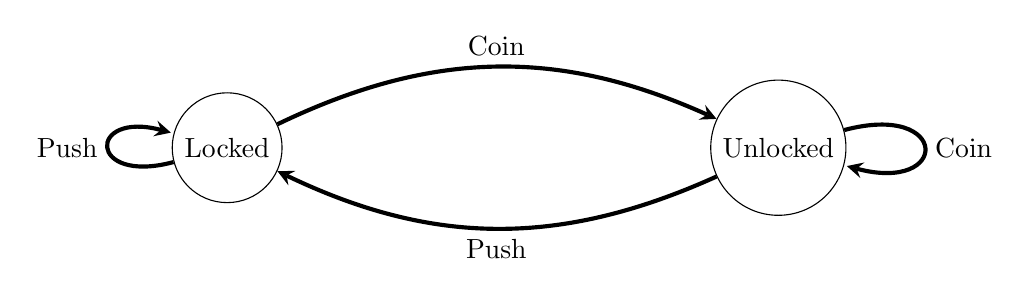
\begin{tikzpicture}[> = stealth,node distance=3cm, on grid]
       \node[state] (q_0) at (-3.5, 0) {Locked};
       \node[state] (q_1) at (3.5, 0) {Unlocked};

       \path[->,line width=1.5] (q_0) edge [loop left] node {Push} ()
           (q_1) edge [loop right] node {Coin} ()
           (q_0) edge [bend left=25, anchor=south] node {Coin} (q_1)
           (q_1) edge [bend left=25, anchor=north] node {Push} (q_0);
   \end{tikzpicture}
   \caption{Турникет}
\end{figure}

\begin{figure}[h]
    \centering
    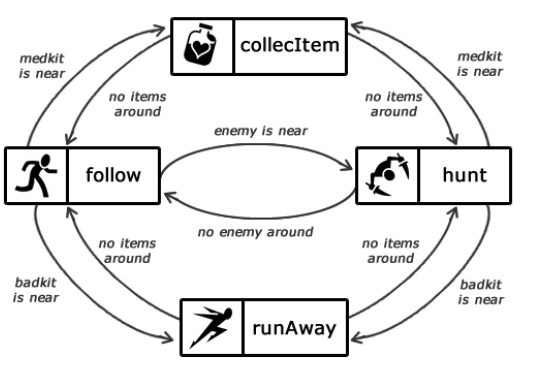
\includegraphics[width=0.6\textwidth]{./img/L2/S002.jpg}
    \caption{Бот}
\end{figure}

\begin{figure}[h]
    \centering
    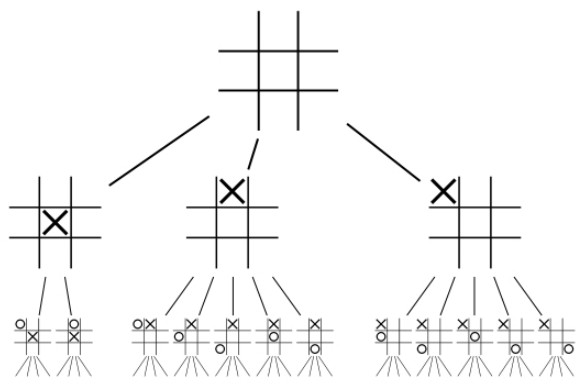
\includegraphics[width=0.6\textwidth]{./img/L2/S003.jpg}
    \caption{Крестики-нолики}
\end{figure}

\FloatBarrier{}

\subsubsection{Определение}
\dfn{(Детерминированный) конечный автомат} --- $ ( Q, \Sigma, \delta, q_0, F ) $ 
\begin{itemize}
    \item $Q \ne 0$ --- конечное множество состояний 
    \item $\Sigma$ --- Конечный входной алфавит
    \item $\delta$ --- отображение типа $Q \times \Sigma \rightarrow Q$\\
    $\delta (q_i, x) = y$
    \item $q_0 \in Q$ --- начальное состояние
    \item $F \subseteq Q$ --- множество конечных состояний
\end{itemize}

Конечный автомат называется \textbf{полным}, если существует переход из каждого состояния по каждому символу алфавита. Если автомат неполный, добавляют \dfn{дьявольскую вершину}

\begin{example}{Дьявольская вершина}
    \[ Q = \{ q_0, q_1, q_2, q_3 \}, \Sigma = \{0, 1, -\}, q_0 = q_0, F = \{ q_1, q_2 \} \]
    \begin{align*}
        \delta(q_0, 0) &= q_1 \\
        \delta(q_0, 1) &= q_2 \\
        \delta(q_0, -) &= q_3 \\
        \delta(q_2, 0) &= q_2 \\
        \delta(q_2, 1) &= q_2 \\
        \delta(q_3, 1) &= q_2
    \end{align*}
    
\end{example}

\begin{figure}[h]
    \centering
    \begin{subfigure}[b]{0.4\textwidth}
        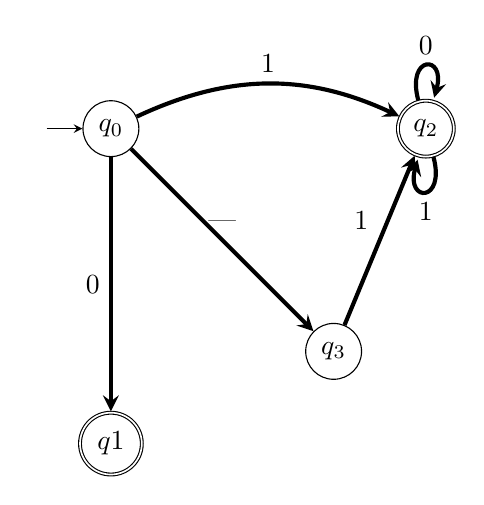
\begin{tikzpicture}[> = stealth,node distance=4cm, on grid]
            \node[state,initial] (q_0) {$q_0$};
            \node[state,accepting] (q_1) [below of=q_0] {$q1$};
            \node[state,accepting] (q_2) [right of=q_0] {$q_2$};
            \node[state] (q_3) [below right of=q_0] {$q_3$};
            \path[->,line width=1.5] (q_0) edge [bend left=25, anchor=south] node {1} (q_2)
                (q_0) edge [anchor=south] node {---} (q_3)
                (q_0) edge [anchor=east] node {0} (q_1)
                (q_3) edge [anchor=south east] node {1} (q_2)
                (q_2) edge [loop above] node {0} ()
                (q_2) edge [loop below] node {1} ();
        \end{tikzpicture}
        \caption{Автомат}
    \end{subfigure}%
    \hspace{2cm}
    \begin{subfigure}[b]{0.4\textwidth}
        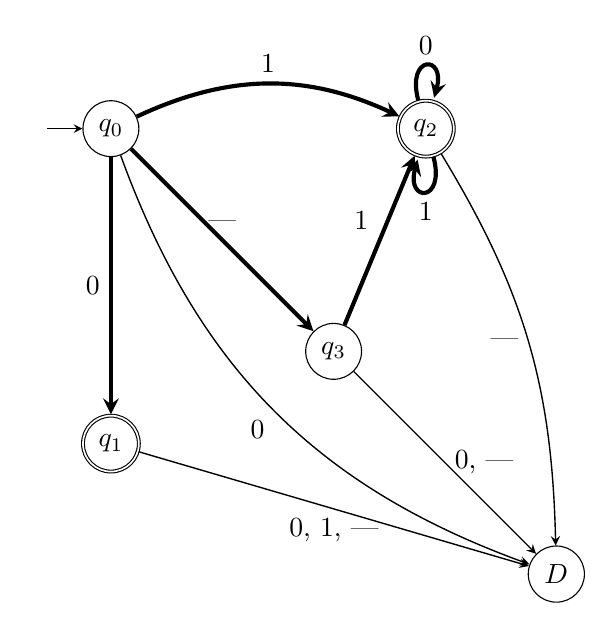
\begin{tikzpicture}[> = stealth,node distance=4cm, on grid]
            \node[state,initial] (q_0) {$q_0$};
            \node[state,accepting] (q_1) [below of=q_0] {$q_1$};
            \node[state,accepting] (q_2) [right of=q_0] {$q_2$};
            \node[state] (q_3) [below right of=q_0] {$q_3$};
            \node[state] (d) [below right of=q_3] {$D$};
            \path[->,line width=1.5]
                (q_0) edge [bend left=25, anchor=south] node {1} (q_2)
                (q_0) edge [anchor=south] node {---} (q_3)
                (q_0) edge [anchor=east] node {0} (q_1)
                (q_3) edge [anchor=south east] node {1} (q_2)
                (q_2) edge [loop above] node {0} ()
                (q_2) edge [loop below] node {1} ();
            \path[->,line width=0.5]
                (q_1) edge [anchor=north] node {0, 1, ---} (d)
                (q_0) edge [anchor=north east, bend right=25] node {0} (d)
                (q_3) edge [anchor=west] node {0, ---} (d)
                (q_2) edge [anchor=east, bend left=15] node {---} (d);
        \end{tikzpicture}
        \caption{Автомат с дьявольской вершиной}
    \end{subfigure}
\end{figure}

\subsubsection{Путь в конечном автомате}
\dfn{Путь} --- кортеж $ \left\langle q_0, e_1, q_1, \ldots, e_n, q_n \right\rangle$
\begin{itemize}
    \item $n \ge 0$
    \item $\forall i: e_i = \left\langle q_{i-1}, w_i, q_i \right\rangle$, где $ \delta(q_{i-1}, w_i) = q_i $
    \item $q_0$ --- \dfn{Начало} пути
    \item $q_n$ --- \dfn{Конец} путь
    \item $w_1, w_2, \ldots w_n$ --- \dfn{Метка} пути
    \item $n$ --- \dfn{Длина} пути 
\end{itemize}


Путь \dfn{успешен}, если $q_0$ --- начальное состояние, а $q_n \in F$ 

Состояние $q$ \dfn{достижимо} из состояния $p$, если существует путь из состояния $p$ в состояние $q$

\subsubsection*{Такт работы КА}
\begin{itemize}
    \item \dfn{Конфигурация (Мгновенное описание)} КА --- $ \left\langle q, \omega \right\rangle$, где $q \in Q, \omega \in \Sigma^* $
    \item \dfn{Такт работы} --- бинарное отношение $\vdash$: если $ \delta(p, x) = q $ и $ \omega \in \Sigma^* $, то $ \left\langle p, x \omega \right\rangle \vdash \left\langle q, \omega \right\rangle $
    \item $\vdash^*$ --- рефлексивное, транзитивное замыкание $\vdash$
\end{itemize}

\subsubsection*{Распознавание слова конечным автоматом}

Цепочка $\omega$ \textit{распознается} КА, если $\exists$ успешный путь с меткой $ \omega $. 

\dfn{Язык, распознаваемый конечным автоматом} --- $ \{ \omega \in \Sigma^* | \exists p \text{ --- успешный путь с меткой } \omega  \} $

\begin{tcolorbox}
    \textbf{Теорема.} Рассмотрим конечный автомат $M = (Q, \Sigma, \delta, q_o, F$).\\
    Слово $\omega \in \Sigma^*$ принадлежит языку $ \Leftrightarrow \exists q \in F: \left\langle q_0, \omega \right\rangle \vdash^* \left\langle q, \varepsilon \right\rangle $
\end{tcolorbox}

Обобщение функции перехода:
\begin{itemize}
    \item $\delta'(q, \varepsilon) = q$
    \item $\delta'(q, x \alpha) = \delta'(\delta'(q, x), \alpha)$, где $x \in \Sigma^*, \alpha \in \Sigma $
\end{itemize}

\begin{tcolorbox}
    \textbf{Теорема}. Цепочка $ \omega $ распознается КА $ \left\langle Q, \Sigma, \delta, q_o, F \right\rangle \Leftrightarrow \exists p \in F: \delta'(q, \omega) = p $
\end{tcolorbox}

\subsubsection*{Свойство конкатенации строк}
\begin{tcolorbox}
    \textbf{Теорема}. $ \left\langle q_1, \alpha \right\rangle \vdash^* \left\langle q_2, \varepsilon \right\rangle, \left\langle q_2, \beta \right\rangle \vdash^* \left\langle q_3, \varepsilon \right\rangle \Rightarrow \left\langle q_1, \alpha\beta \right\rangle \vdash^* \left\langle q_3, \varepsilon \right\rangle  $
\end{tcolorbox}

\subsubsection{Эквивалетность конечных автоматов}
Конечные автоматы $A_1, A_2$ \dfn{эквивалетны}, если распознают один и тот же язык.

Проверка на эквивалентность --- одновременный обход в ширину двух автоматов. Каждый переход должен приводить в терминальне или нетерминальные вершины в обоих автоматах соответственно

\dfn{Минимальный конечный автомат} --- автомат, имеющий наименьшее число состояний, распознающий тот же язык, что и данный. 

\subsubsection{Классы эквивалетности}
\dfn{Отношение эквивалетности} --- рефлексивное, симметричное, транзитивное отношение
\begin{itemize}
    \item $xRx$
    \item $xRy \Longleftrightarrow yRx$
    \item $xRy, yRz \Rightarrow xRz$
\end{itemize}

\begin{tcolorbox}
    \textbf{Теорема}. $\forall R$ --- отношение эквивалентности на множестве $S$\\
    Можно разбить $S$ на $k$ непересекающихся подмножеств подмножеств $I_1, \ldots, I_k$, т.ч. $aRb \Leftrightarrow a, b \in I_j$
\end{tcolorbox}
Множества $I_1 \ldots I_k$ называются \dfn{классами эквивалетности}

\subsubsection*{Эквивалетные состояния}
\begin{itemize}
    \item $\omega \in \Sigma^*$ \dfn{различает} состояния $q_i$ и $q_j$, если $\delta'(q_i, \omega) = t_1$, $\delta'(q_j, \omega) = t_2 \Rightarrow (t_1 \notin F \Leftrightarrow t_2 \in F )$
    \item $q_i, q_j$ \dfn{эквиваленты}, $(q_i ~ q_j)$, если $\forall \omega \in \Sigma^*$: $\delta'(q_i, \omega) = t_1, \delta'(q_j, \omega) = t_2 \Rightarrow (t_1 \in F \Leftrightarrow t_2 \in F)$
\end{itemize}

\begin{tcolorbox}
    \textbf{Лемма}. $A = \left\langle Q, \Sigma, \delta, q_0, F \right\rangle, p_1, p_2, q_1, q_2 \in Q, q_i = \delta(p_i, c) $. $ \omega \in \Sigma^* $ различается $q_1$ и $q_2$. Тогда $c\omega$ различает $p_1$ и $p_2$.
\end{tcolorbox}

\begin{tcolorbox}
    \textbf{Доказательство}. $ \delta'(p_i, c \omega) = \delta'( \delta'(p_i, c), \omega ) = \delta'(q_i, \omega) = t_i $ 
\end{tcolorbox}

\subsubsection*{Алгоритм минимизации} % TODO
\begin{itemize}
    \item $Q$ --- очередь
    \item \texttt{marked} --- таблица размером $n \times n$
\end{itemize}

Пустой цепочкой различимы конечные и неконечные состояния

\subsection{Недетерминированный КА}
Отличается отображение. Из состояния по символу происходит переход в некоторое множество состояний. В графическом виде это значит, что из одной вершины по одному символу выходит одна или несколько стрелок.

Такт работы связывает две конфигурации

ДКА --- частный случай НКА. В множестве может быть и один элемент

ДКА строить сложнее, но их легче использовать --- если длина цепочки $n$, то можно проверить, принадлежит ли она языку за $o(n)$.

\end{document}
